\documentclass[12pt]{article}

\usepackage[a4paper,margin=2.5cm]{geometry}
\usepackage{amsmath, amssymb, amsthm}
\usepackage{bm}
\usepackage{hyperref}
\usepackage{graphicx}
\usepackage{caption}
\usepackage{listings}
\usepackage{xcolor}
\usepackage{float}
\usepackage{placeins}
\graphicspath{{figures/}}

\lstdefinestyle{code}{
  basicstyle=\ttfamily\small,
  numbers=left,
  numberstyle=\tiny,
  numbersep=8pt,
  keywordstyle=\color{blue},
  commentstyle=\color{teal!70!black},
  stringstyle=\color{orange!70!black},
  showstringspaces=false,
  breaklines=true,
  frame=single,
  framerule=0.3pt,
  rulecolor=\\color{black!15}
}
\lstset{style=code}

\title{Principal Component Analysis Tutorial}
\author{}
\date{\today}

\begin{document}
\maketitle

\section{Introduction}
Principal Component Analysis (PCA) seeks orthogonal directions that capture maximal variance, providing dimensionality reduction, visualization, and noise suppression for numerical data. By projecting observations onto a low-dimensional subspace spanned by top principal components, PCA yields compact representations while preserving dominant structure.

\section{Theory and Formulas}
\subsection{Covariance Matrix and Eigendecomposition}
Given centered data matrix \(\mathbf{X} \in \mathbb{R}^{n \times d}\), the empirical covariance is
\begin{equation}
\mathbf{S} = \frac{1}{n-1} \mathbf{X}^\top \mathbf{X}.
\end{equation}
PCA solves the eigenvalue problem \(\mathbf{S}\mathbf{u}_k = \lambda_k \mathbf{u}_k\) with \(\lambda_1 \ge \lambda_2 \ge \cdots \ge 0\). The \(k\)-dimensional principal subspace is spanned by \(\mathbf{U}_k = [\mathbf{u}_1, \dots, \mathbf{u}_k]\).

\subsection{Projection and Reconstruction}
Projected scores (principal components) are given by
\begin{equation}
\mathbf{Z} = \mathbf{X} \mathbf{U}_k,
\end{equation}
while the rank-\(k\) reconstruction is \(\hat{\mathbf{X}} = \mathbf{Z}\mathbf{U}_k^\top\). The fraction of variance explained by the first \(k\) components equals
\begin{equation}
\text{ExplainedVariance}(k) = \frac{\sum_{i=1}^k \lambda_i}{\sum_{j=1}^d \lambda_j}.
\end{equation}

\subsection{Singular Value Decomposition View}
PCA can also be expressed through SVD: \(\mathbf{X} = \mathbf{U}\mathbf{\Sigma}\mathbf{V}^\top\). Columns of \(\mathbf{V}\) are eigenvectors of \(\mathbf{S}\); singular values satisfy \(\sigma_i^2 = (n-1)\lambda_i\). This perspective supports efficient computation for high-dimensional data.

\section{Applications and Tips}
\begin{itemize}
  \item \textbf{Visualization}: project high-dimensional data to two or three principal components to reveal clusters or trends.
  \item \textbf{Preprocessing}: reduce dimensionality before clustering or regression to mitigate multicollinearity and noise.
  \item \textbf{Compression}: store only principal scores and loadings for recommender systems or image compression pipelines.
  \item \textbf{Best practices}: center features, optionally scale to unit variance, inspect explained variance curves, and monitor for component flipping when interpreting axes.
\end{itemize}

\section{Python Practice}
The script \texttt{gen\_pca\_figures.py} generates a synthetic dataset with correlated features, fits PCA, and saves both a projection plot and an explained-variance curve.
\begin{lstlisting}[language=Python,caption={Excerpt from gen_pca_figures.py}]
from sklearn.decomposition import PCA

pca = PCA(n_components=3, whiten=False, random_state=7)
pca.fit(points)
projected = pca.transform(points)

explained = np.cumsum(pca.explained_variance_ratio_)
\end{lstlisting}

\section{Result}
\begin{figure}[H]
  \centering
  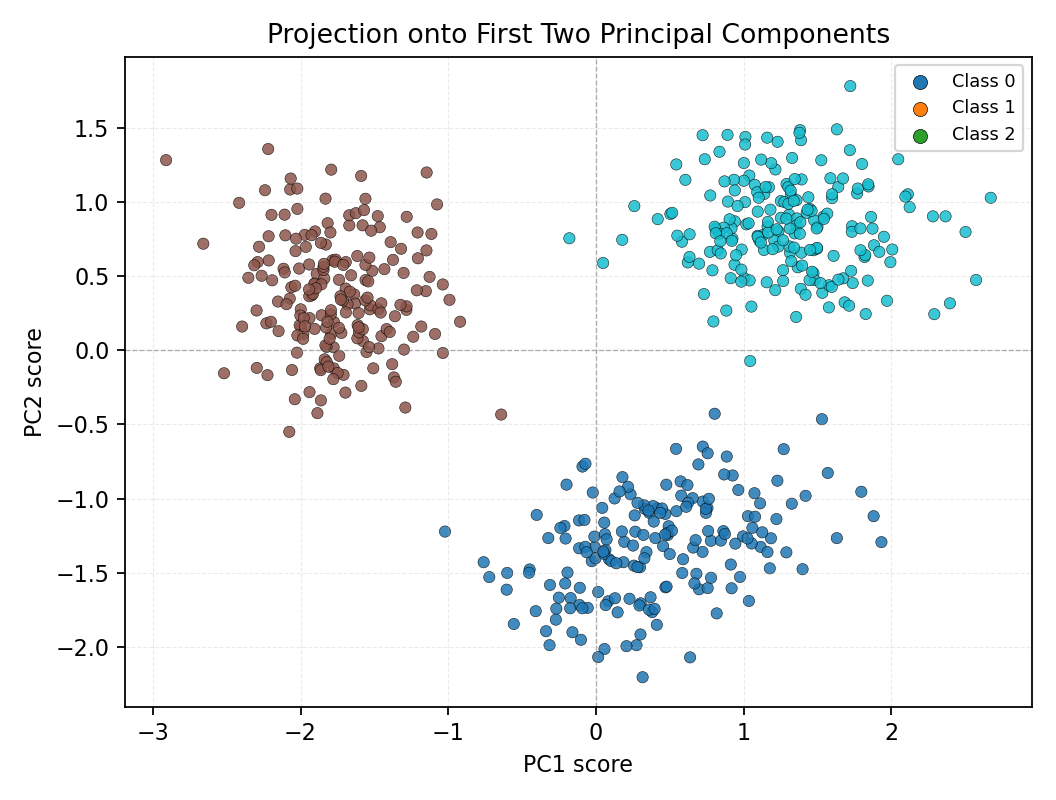
\includegraphics[width=0.82\linewidth]{pca_projection.png}
  \caption{Scatter of the first two principal components with class colors}
  \label{fig:pca_projection}
\end{figure}

\begin{figure}[H]
  \centering
  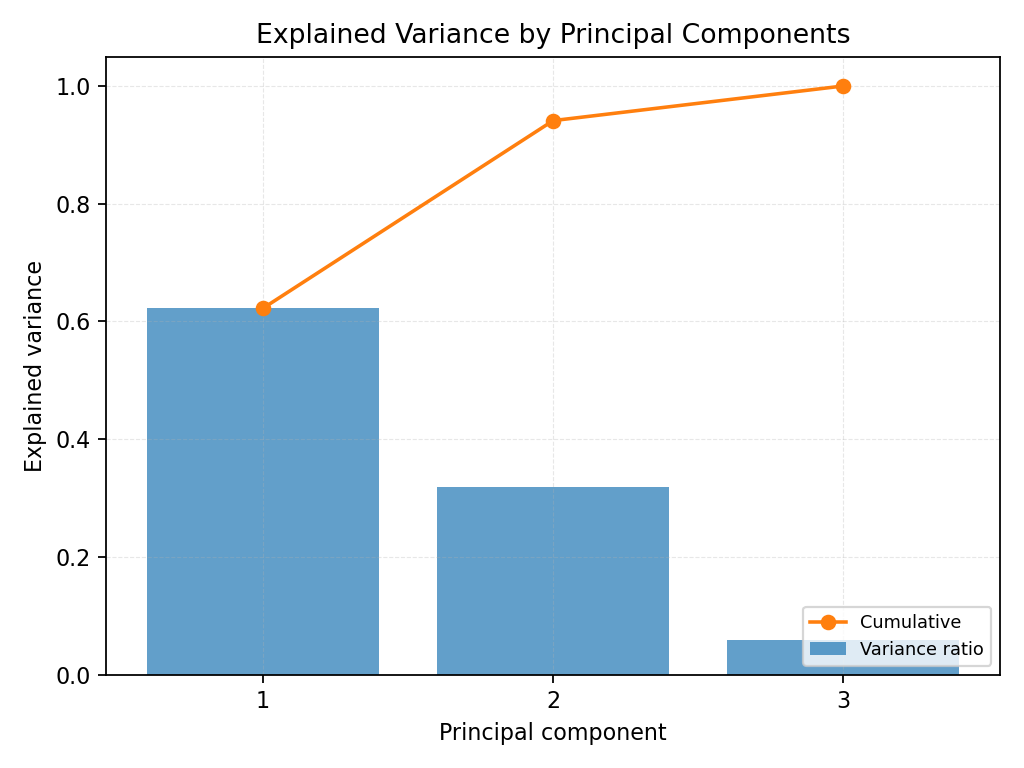
\includegraphics[width=0.8\linewidth]{pca_explained_variance.png}
  \caption{Explained variance ratio and cumulative curve across components}
  \label{fig:pca_explained_variance}
\end{figure}

\FloatBarrier
\section{Summary}
PCA extracts orthogonal directions of maximal variance via eigenvalue decomposition or SVD. Low-dimensional projections and explained variance diagnostics enable practitioners to balance compression with information retention. The synthetic example illustrates how scatter plots of principal scores and variance curves guide component selection.

\end{document}




